% Quelques mots sur le metier:
% + rappel sur les fonctions
% + rappel sur les distributions
% + rappel sur les convergences
% + rappel sur les stats
\documentclass[8pt]{beamer}

\setbeamertemplate{background canvas}[vertical shading][bottom=cyan!10,top=blue!10]

\usetheme{Warsaw}
\usefonttheme[onlysmall]{structurebold}

% pour le fichiers .pdf
\usepackage{graphicx}
\usepackage{color}
% pour les fichiers .png
% \usepackage{pgf,pgfarrows}
% \usepackage{pgf,pgfarrows}
\usepackage{amsmath,amssymb}
\usepackage{textcomp}
\usepackage{Math_Notations}
\usepackage{multitoc}
\usepackage{mdwtab}
\setbeamercovered{dynamic}
\DeclareMathOperator*{\argmin}{argmin}

\title[OpenTURNS Developer Training]{OpenTURNS Developer Training\\Probabilistic uncertainty propagation}
\author[OpenTURNS Consortium, 2019]{
  Trainer : R\'egis LEBRUN, Airbus
  regis.lebrun@iairbus.com
}

\date[March 22-25th 2011]{
  Developers training \\

  \begin{center}
    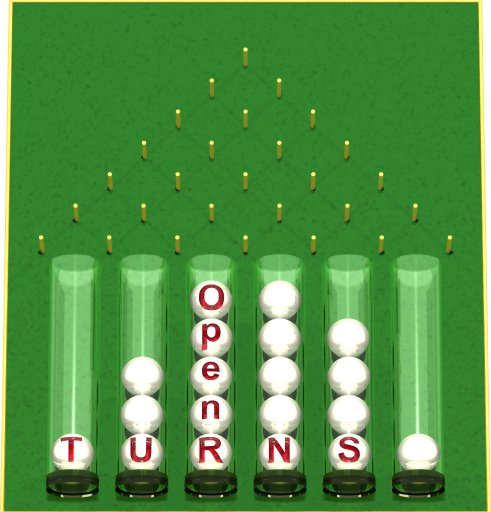
\includegraphics[height=2cm]{logoOT.jpg}
  \end{center}

}

\subject{OpenTURNS Developers Training}

% \part<presentation>{Corps de presentation}


\begin{document}

\frame{\titlepage}

% necessaire pour la table des matieres
\part{Main part}

% table des matieres
\begin{frame}
  \frametitle{OpenTURNS Developers Training Overview}
  \tableofcontents[part=1]
\end{frame}
%%%%%%%%%%%%%%%%%%%%%%%%%%% 
% Uncertainty propagation %
%%%%%%%%%%%%%%%%%%%%%%%%%%% 
\section[What is uncertainty propagation?]{What is uncertainty propagation?}
%%%%%%%%%%%%%%%%%% 
% Main objective %
%%%%%%%%%%%%%%%%%% 
\begin{frame}
  \frametitle{Main objective}
  \begin{block}{Probabilistic uncertainty propagation}
    OpenTURNS = Open Source Treatment of Uncertainty, Risk'N Statistics
    \begin{itemize}
    \item Uncertainty = unknown quantities, lack of exact knowledge, non predictible fluctuations
    \item Risk = dangerous state, critical conditions and their impact (cost, consequences)
    \item Statistics = observation and modelling of random quantities, partial knowledge
    \item Treatment = algorithmic tools to analyse, model and quantify the previous points
    \end{itemize}
    The main objective of OpenTURNS is to quantify and analyse a critical \emph{event $E$} built upon a \emph{quantity of interest $Y$} that is linked to \emph{sources of uncertainty $\vect{X}$} through a \emph{numerical model $f$}:
    \begin{equation}
      E=\mathbf{1}_{Y>s}\quad,Y=f(\vect{X})
    \end{equation}
    where $s\in\R$ is a given threshold, $\vect{X}$ is a random vector, $E$ is the critical event. The quantification of this event is typically the evaluation of its \emph{probability of occurence $\P(E)$}.
  \end{block}
\end{frame}
%%%%%%%%%%%%%%%%%%% 
% Numerical model %
%%%%%%%%%%%%%%%%%%% 
\begin{frame}
  \frametitle{Numerical models}
  \begin{block}{OpenTURNS concept}
    Mathematically speaking, a \emph{numerical model $f$} is a function defined over a subset of $\R^n$ and taking values in a subset of $\R^p$. In OpenTURNS, such a concept is implemented by the \emph{NumericalMathFunction} class. This class proposes 3 main services:
    \begin{itemize}
    \item An \emph{evaluation} method: for all vector $\vect{x}\in\R^n$, a NumericalMathFunction must either compute the value of $f(\vect{x})$ if it is well defined, or throw an exception. \emph{Warning: the domain of definition of $f$ is only implicitely known.}. The evaluation is delegated to the \emph{NumericalMathEvaluationImplementation} class, which is a \emph{mandatory} part of the NumericalMathFunction.
    \item A \emph{gradient} method: for all vector $\vect{x}\in\R^n$, a NumericalMathFunction may compute the value of $\nabla f(\vect{x})\in\mathcal{M}_{n,p}(\R)$ if it is well defined, or throw an exception. The gradient computation is delegated to the \emph{NumericalMathGradientImplementation} class, which is an \emph{optional} part of the NumericalMathFunction.
    \item An \emph{hessian} method: for all vector $\vect{x}\in\R^n$, a NumericalMathFunction may compute the value of $\nabla^2 f(\vect{x})\in\mathcal{T}_{n,n,p}(\R)$ if it is well defined, or throw an exception. The hessian computation is delegated to the \emph{NumericalMathHessianImplementation} class, which is an \emph{optional} part of the NumericalMathFunction.
    \end{itemize}
  \end{block}
  This concept is refined in several sub-classes in a hierarchy that is one of the key part of OpenTURNS.
\end{frame}
%%%%%%%%%%%%%%%%%%%%%%%%%%%%%%%%%% 
% Distribution and random vector %
%%%%%%%%%%%%%%%%%%%%%%%%%%%%%%%%%% 
\begin{frame}
  \frametitle{Random vector, distribution}
  \begin{block}{Definition}
    A \alert{random vector $\vect{X}$} is a measurable function from a probability space $(\Omega, \mathcal{B}(\Omega), \P)$ into a numerical space $\R^n$. The associated \alert{distribution} is the probability measure $\mu_{\vect{X}}$ defined by $\forall B\in\mathcal{B}(\R), \mu_{\vect{X}}(B)=\P(\vect{X}^{-1}(B))$. The different values $\vect{X}(\omega)$ taken by a random vector $\vect{X}$ are called the \alert{realizations} of the random vector.
  \end{block}
  \begin{block}{Main properties}
    \begin{itemize}
    \item a random vector generates realizations (\alert{RandomVector::getRealization()})
    \item a distribution computes probabilities (\alert{Distribution::computeCDF()})
    \end{itemize}
  \end{block}
\end{frame}
%%%%%%%%%%%%%%%%%%%%%%%%% 
% The Uncertainty layer %
%%%%%%%%%%%%%%%%%%%%%%%%% 
\begin{frame}
  \frametitle{The Uncertainty layer}
  \begin{block}{}
  \end{block}
\end{frame}
%%%%%%%%%%%%%%%%%%%%%%%%%%%%%%%%%%%% 
% Where to place your development? %
%%%%%%%%%%%%%%%%%%%%%%%%%%%%%%%%%%%% 
\begin{frame}
  \frametitle{Where to place your development?}
  \begin{block}{}
  \end{block}
\end{frame}

\end{document}

